%!TEX root = ../../FYP_Dissertation.tex

When looking at the timing of individual tests of the MAD test suite we can see
that most of the instability comes from the Model Object tests. In Figure
\ref{fig:failed-test}, we can see a screenshot of three failed timing tests that
were calibrated to run in roughly 0.5 seconds and that for this run needed respectively
6, 4 and 68 seconds. We need then to investigate the reason for such results.

\begin{figure}[H]
    \centering
	\includegraphics[width=0.8\textwidth]{./Images/failed-test.png}
    \caption{Timing screenshot}
    \label{fig:failed-test}
\end{figure}

The Lua programming language doesn't actually have an object model but provide
mechanisms that allow anyone to build a custom object model fitting his needs.
Next section will present the one that as been built for MAD.

%===============================================================================
% Model object description
%===============================================================================

\section{Model object description}
\label{Sec:MO-descriptinon}

MAD object module implements the necessary machinery to support prototype-based
programming. When reading an attribute on an object, either the value is present
in the child object and it is returned or the query is passed to the parent
object recursively until the value is found or the original \emph{Object} is
reached. When a value is written the value is simply stored in the current
object (no lookups are performed). To understand how this object model is
implemented, a grasp of how lua handles tables and metatables is required.

To keep it simple here, lua tables are key-value stores that return \emph{nil} by
default if a key is not defined (see Section \ref{Subsec:table} for more).
Users have the possibility to associate a metatable to any tables. A metatable
is actually a standard lua table that contains special metamethods of which
the keys are defined by the lua language. The one that we are interested here is
the \emph{\_\_index} metamethod that defines how a table should react when accessing
an undefined key. If this is a method, the requested key is passed to this method
and it is executed, but if this \emph{\_\_index} contains another table, then this
table is queried instead of the first one. This is this mechanism that has been
used in MAD to implement the model object. Figure \ref{fig:MO-descriptinon} below
shows a schematic of the implementation of MAD object model.

\begin{figure}[H]
    \centering
    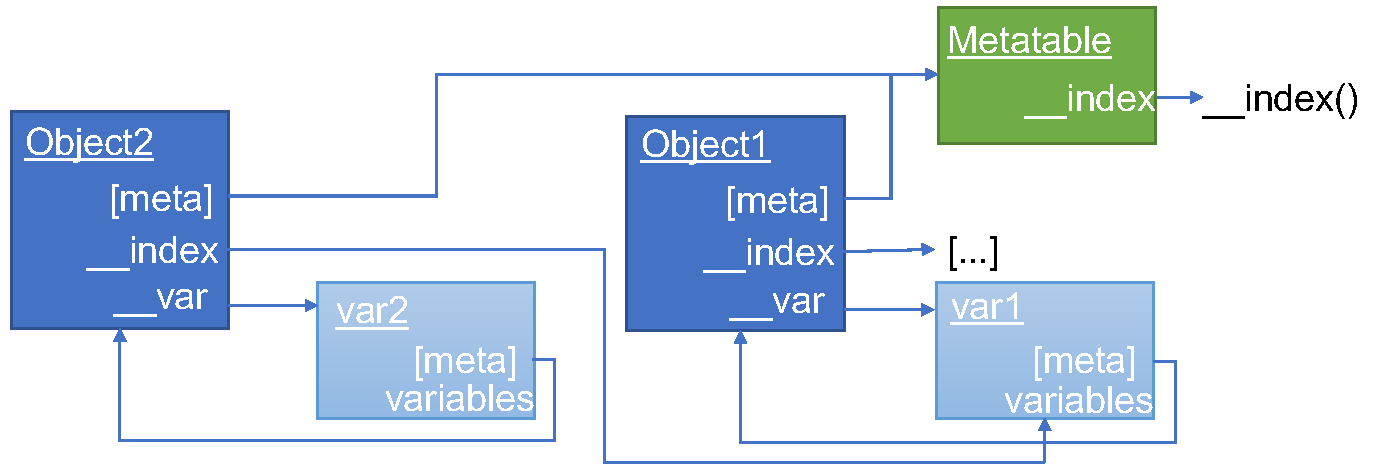
\includegraphics[width=\textwidth]{./Images/MO.pdf}
    \caption{Implementation of MAD object model}
    \label{fig:MO-descriptinon}
\end{figure}

On this figure, \emph{Object2} is the child of \emph{Object1}. To represent an
object, three lua tables are actually needed. The first one (in dark blue) is
the actual object passed around and manipulated by the user. It doesn't actually
contain any user data so when queried, the index function of its metatable (in
green) is executed instead. This metatable is by default the same for all objects
unless it is explicitly modified by the user. This index function gets the
\emph{var} table (in light blue) of the object and try to index it with the
requested key. If the key is defined, the corresponding value is returned,
otherwise the chaining lookup is triggered. Let's look at the example in the
figure when trying to query an undefined key in \emph{Object2}.
First the index function query \emph{var2} that doesn't contain it. Then, since
\emph{Object2} is the metatable of \emph{var2} (see the \emph{[meta]} arrow) and
the \emph{\_\_index} of \emph{Object2} links to \emph{var1}, \emph{var1} is queried.
This chaining is done recursively to the \emph{var} tables of its parents until the
key is found or the hierarchy entirely unrolled.

%===============================================================================
% Performance analysis
%===============================================================================

\section{Performance analysis and possible explanation}
\label{Sec:MO-perf-analys}

%
% - performance issue
%	- possible explanation
%   - show trace
%   - explane how the JIT was in mind when develloping this object model
%     and how it fall.
%     explan how normally it should work with a single small example
%     mention hosting and loop optimization
% loop optimization is a problem here when the list is heterogenous in numbers of stages
%  permanant blacklisting
% removing blacklisting after a flush
% allow blacklisted function and or
%   - but not triggers a compilation

%===============================================================================
% Performance of Sequence iterator
%===============================================================================

\section{Performance of \emph{Sequence} iterator}
\label{Sec:MO-perf-iter}

% forward vs backward iterator
% difference in performance
% comming from the nedd of the l
	% different depth to get l
	% show a visual dump
% new object model ?

%===============================================================================
% Model object alternative design
%===============================================================================

\section{Model object alternative design}
\label{Sec:MO-alt-design}

% exploration of other type of object model
%  performance compareson / explanation
% didn't help on average